
\chapter{DScalaness/DnesT}
\label{chapter-dscalaness-dnest}

% Theory from the CC and GPCE papers...

In this chapter I describe a staged programming language system supporting type safe dynamic
code generation for resource constrained embedded devices. This system features programming
abstractions for specializing device code and allowing on-the-fly adaptation to current device
deployment conditions. The system has been implemented as an extension to Scala \cite{PiS2},
through modification of the Scala compiler.

I specifically consider scenarios where a relatively powerful hub device can automatically
combine dynamically specialized libraries and deploy them to a wireless sensor network using
some over-the-air deployment method such as Deluge \cite{deluge04}. To this end a restricted
form of staging \cite{Taha-MetaML,DBLP:conf/icess/Taha04,289140} is used to achieve well founded
dynamic program generation. \emph{First stage} code is written in an extended version of Scala,
called Scalaness, which is programmer friendly and suitable for running on powerful hubs. The
execution of a Scalaness program yields a residual \emph{second stage} node program written in
nesT, a type safe variant of the nesC programming language. The second stage program is
constructed from module components treated as first class values, which may be type and value
specialized during the course of first stage computation.

\autoref{figure-scalaness} provides an overview of the Scalaness/nesT language architecture.
Scalaness source code is compiled in a modified Scala compiler to Java bytecode, and run in a
standard Java virtual machine (JVM). At runtime this Scalaness program may generate nesT code,
which is subsequently rewritten to nesC and compiled using the standard TinyOS compiler. The
resulting image can then be installed on sensor network nodes.

\begin{fpfig*}[t]
  {Scalaness/nesT Compilation and Execution Model}
  {figure-scalaness}
  %\hspace{0mm}
  \begin{center}
    % \includegraphics[scale=.565]{scalaness}
    \includegraphics[scale=.54]{Figures/scalaness.eps}
  \end{center}
\end{fpfig*}

Since the Scalaness program has at its disposal the resources and features of the full Scala
environment, including the JVM and its associated libraries, there are few limitations imposed
on the first stage program. It could, at the programmer's option, generate separate images for
each node on the sensor network or regenerate the node images at a later time to account for
evolving network behavior.

Another interesting feature of the architecture, captured in \autoref{figure-scalaness}, is the
physical platform on which different elements of the Scalaness/nesT ``workflow'' may be
executed. Scalaness source code will typically be compiled in the lab, prior to deployment but
execution of the Scalaness program may be done on a separate device in the field where the user
will not be in a position to fix type errors in the generated images.

Consequently a central contribution of Scalaness is static type safety. In particular, the
Scalaness type system ensures that typeable Scalaness programs will always generate type safe
residual nesT program. Since type generalization is allowed to be cross-stage, the technology
supports a novel form of cross-stage type specialization. In existing strongly typed staged
sensor programming environments the type correctness of second stage programs must be verified
after execution of first stage code \cite{Mainland-Flask-2008}, and could in fact produce an
error which would invalidate the deployment. Such type errors are always caught at first stage
compilation time with Scalaness. Previous work on the staged programming calculus $\langle
\text{ML} \rangle$ \cite{FramedML} provides a theoretical foundation for Scalaness/nesT type
safety.

Both Scala and nesC are complex, industrial strength languages. Neither of them are fully
formalized. Thus in order to effectively study the Scalaness/nesT staged programming system, it
is useful to consider simplified or ``distilled'' versions of those languages. Here I use the
names Scalaness and nesT to refer to the languages as implemented and \newterm{DScalaness} and
\newterm{DnesT} to refer to the distilled languages studied theoretically. The implementation is
described in more detail in \autoref{chapter-scalaness-nest}. The distilled languages are
described in this chapter.

\section{Overview of DScalaness/DnesT Design}

The goal of DScalaness/DnesT is to describe a practical programming system for writing arbitrary
embedded applications. In that respect it is more general than SpartanRPC, which focuses on the
specific problems of providing a convenient RPC discpline together with language level features
for controlling resource access. In contrast, authorization is only one application of many to
which Scalaness/nesT could be applied.

Scala is an appropriate choice as a basis for the first stage language because its compiler is
open source and easy to modify and maintain. Also Scala offers a rich, flexible, and user
friendly set of features familiar to application programmers working in traditional (desktop,
server) environments. Finally Scala has an active user community with a growing collection of
tools and other supporting resources.

However, Scala is not appropriate in the extremely resource constrained environment of a sensor
network node or other small embedded system. In contrast nesT is implemented by translation into
nesC, which can in turn be compiled for TinyOS platforms. The nesT language is roughly (although
not exactly) a subset of nesC and shares with nesC many features appropriate for embedded
systems programming.

To demonstrate DScalaness and DnesT I will show an example that illustrates both type and value
specialization of DnesT modules. Although the example is small it nevertheless demonstrates the
essential features of the system in a suggestive manner.

It is well-known that minimizing the number of bits used to represent a sensor node address can
produce significant energy savings. Each bit of transmission consumes energy similar to 800
instructions \cite{tag} so the fewer bits transmitted the better. However, sensor networks are
``ad hoc'' in the sense that the distribution of the nodes is often unpredictable until
deployment, so the optimal data type used to represent node addresses is an environmental
property that may need to be determined \emph{in situ}.

The example also value specializes DnesT modules with specific session keys for use during
secure communication. In previous work I showed how symmetric key message authentication codes
can be used to support resource authorization in sensor networks
\cite{chapin-skalka-SpartanRPC,chapin-skalka-SpartanRPCTR}. In particular, communication between
security domains in a sensor network can be mediated by credentials implemented as keys, with
nodes lying at domain frontiers using different keys to send (to the other domain) and receive
(from the other domain) over secured links. Since it is unpredictable where nodes will be
physically distributed in space, appropriate keys for each node need to be established \emph{in
  situ}. Defining node functionality using generic code that must be instantiated with specific
keys allows adaptation to a deployment environment, and allows expensive computations for
establishing session keys to be offloaded from the network nodes to a higher powered device.

\autoref{figure-example} shows the complete example. We begin with the definition of a
parameterized type $\tt{mesgT(t)}$ using the DScalaness $\tt{abbrvt}$ binder, where an instance
$\tt{mesgT}(\t)$ denotes the ground type obtained by substituting $\t$ for $\tt{t}$ in the
definition of $\tt{mesgT}$.

% TODO: The formatting of this example could be improved (notice inconsistent font size).
\begin{fpfig}[!p]{DScalaness/DnesT Example}{figure-example}
{
\singlespace
\lstset{numbers=left, numberstyle=\tiny, numbersep=0pt, basicstyle=\ttfamily}
\lstset{escapeinside={(*@}{@*)}}
\begin{lstlisting}
 (*@\tt{abbrvt\ mesgT(t)\  =}@*) { src : (*@\tt{t}@*); dest : (*@\tt{t}@*); data : uint8[] };  (*@\label{l:mesgt}@*)

 (*@\tt{abbrvt\ radioT\  =}@*) < mt (*@$\subtype$@*) (*@\tt{mesgT}@*)(uint) > (*@\label{l:radiot}@*)
                 { export error_t radio_x(mt*); 
                   import error_t handle_radio_r(mt*); };

 (*@\tt{abbrvt\ commT\ \  =}@*) (mt (*@$\subtype$@*) (*@\tt{mesgT}@*)(uint)) (*@$\circ$@*) (*@\label{l:commt}@*)
                 < >
                 { export error_t send(mt*); 
                   import error_t handle_receive(mt*); };

 (*@\tt{authSend\ \  =}@*) < mt (*@$\subtype$@*) (*@\tt{mesgT}@*)(uint);(*@\label{l:authsend}@*) sendk : uint8[],>  
             { import error_t radio_x(mt*);
               export error_t send(m : mt*) 
                      { radio_x(AES_sign(m, sendk)); } };

 (*@\tt{authRecv\ \  =}@*) < mt (*@$\subtype$@*) (*@\tt{mesgT}@*)(uint);(*@\label{l:authrecv}@*) recvk : uint8[] >  
             { import error_t handle_recv(mt*);
               export error_t handle_radio_r(m : mt*) 
                      { if AES_signed(m, recvk) 
                         handle_recv(m); } }; 

 (*@\tt{def\ authSpecialize}@*) (*@\label{l:authspecialize}@*)
  (*@ \tt{(nmax : uint16, radioM : radioT, keys : uint8[][]) : commT }@*) { (*@\label{l:args}@*)
     (*@\tt{typedef\ adt \subtype uint = \ if\ (nmax  \le 256)\ uint8\ else\ uint16;}@*)  (*@\label{l:typedef}@*) 
     (*@\tt{val\ sendM = \jinst{authSend}{mesgT(adt); keys[0]};}@*)  (*@\label{l:inst1}@*)
     (*@\tt{val\ recvM = \jinst{authRecv}{mesgT(adt); keys[1]};}@*)  (*@\label{l:inst2}@*)    
     (*@\tt{(sendM \ltimes \jinst{radioM}{mesgT(adt)}) \ltimes recvM;}@*) (*@\label{l:wire}@*)
    }

 (*@\tt{appMR\ =}@*) (*@\label{l:main}@*)
  < > { export handle_recv(m : (*@\tt{mesgT}@*)(uint8)*) {(*@\ldots@*)} }; 
 (*@\tt{appM\ =}@*) 
  < > { import send((*@\tt{mesgT}@*)(uint8)*); export main() {(*@\ldots@*)} };  
 (*@\tt{image(appM \ltimes (authSpecialize(nmax, radioM, keys) \ltimes appMR)); } @*) (*@\label{l:image}@*)  
\end{lstlisting}
\primaryspacing
}
\end{fpfig}


Next, on line~\ref{l:radiot} we define a type $\tt{radioT}$, which is the type of DnesT modules
that provide an API to the radio. The DnesT module language is a simplified version of the nesC
component language. In this example, any module of type $\tt{radioT}$ exports a $\tt{radio\_x}$
function for sending messages, and imports a $\tt{handle\_radio\_r}$ function that allows
received messages to be handled in a user-defined manner. Both functions take message references
as arguments. Furthermore, the module is parameterized by the type of messages $\tt{mt}$, where
the address type is upper-bounded by 32-bit unsigned integer. Thus, any module of type
$\tt{radioT}$ can be dynamically specialized to a 32, 16, or 8 bit address space. Module type
parameters are always defined with brackets $\tt{<...>}$.
 
Now on line~\ref{l:commt} we define another type $\tt{commT}$ which is the type of modules
providing a QOS layer over a specialized radio. Although this type is also parameterized by a
bounded message type $\tt{mt}$, as is $\tt{radioT}$, the parameterization is subtly different
syntactically and semantically, since $\tt{commT}$ expects a program context where the radio has
been specialized. Thus, in $\tt{commT}$, $\tt{mt}$ is understood as being ``some'' type with an
upper bound of $\tt{mesgT(uint)}$ which occurs in the module signature, whereas the module
itself has no parameters to be instantiated. This sort of type is needed in the presence of
\emph{dynamic type construction}.

Next on lines \ref{l:authsend} and \ref{l:authrecv} we define modules for sending and receiving
messages that provide a layer of authentication security over the radio. Observe that in the
implementation of $\tt{send}$ in module \tt{authSend}, messages are signed with a key
$\tt{sendk}$, whereas when messages are received they must be signed with a possibly different
key $\tt{recvk}$ before being passed on to the user's receive handler, as specified in module
\tt{authRecv}. These modules are parameterized by a message type $\tt{mt}$, and also the
$\tt{sendk}$ and $\tt{recvk}$ key values.

To generalize a technique for composing these modules with a radio to yield a module of type
\tt{commT}, that is abstract with respect to neighborhood sizes, radio implementations, and
session key material, the DScalaness $\tt{authSpecialize}$ function is defined on
line~\ref{l:authspecialize}. The first-class status of DnesT modules in DScalaness is apparent
here. On line~\ref{l:args} the function is specified to take a module parameter $\tt{radioM}$ of
type $\tt{radioT}$ among its arguments, and to return a module of type $\tt{commT}$ as a result.
It also takes an array of keys as an argument, and on lines~\ref{l:inst1} and~\ref{l:inst2} it
instantiates $\tt{sendMesg}$ and $\tt{recvMesg}$ with the keys in the array. Finally it uses the
type $\tt{adt}$ in the instantiations, which in line~\ref{l:typedef} is dynamically constructed
on the basis of the input variable $\tt{nmax}$.

This illustrates a key novelty of the system, the ability to \emph{dynamically} set a type to
use on a node based on a decision made during the execution of the DScalaness program. Since the
value of $\tt{nmax}$ cannot be statically determined, the type analysis only knows that
$\tt{adt}$ is some subtype of $\tt{uint}$. Finally, on line~\ref{l:wire} the instantiated radio
module is composed with the instantiated send and receive modules via the DScalaness $\ltimes$
operator. The semantics of module composition here is standard \cite{Cardelli-1997}; in a
composition aka wiring $\mu_1 \ltimes \mu_2$, the exports of $\mu_2$ are connected to imports of
$\mu_1$. The function result is a module of type \tt{commT}.

To obtain a module defining a mote OS image in a program context where neighborhood size is
known, a radio implementation has been provided, and session keys have been computed. We can
then compose the results of an \tt{authSpecialize} function with modules specifying top-level
message send and receive behaviors, and a \texttt{main} application entry point (here we assume
it is known that address sizes can be limited to 8 bits, so \tt{nmax} < 256). At line
\ref{l:image} a closed module is defined and a binary mote image can be produced by a call to
\tt{image}.

In DScalaness, \tt{image} is an assertion that its argument is a \emph{runnable} module, with no
unresolved parameters or imports. In the Scalaness implementation, this is the point where nesT
source code is actually generated. Successful DScalaness/DnesT type checking (which occurs
during stage 1 compilation as per \autoref{figure-scalaness}) statically guarantees that
specialized code generated at the point of \tt{image} will run in a type-safe manner when it is
eventually loaded and run on a node.

\subsection{Modules as Staging Elements}

In DScalaness, DnesT modules can be treated as data to be composed, following traditional staged
programming languages \cite{Taha-MetaML}. The so-called ``runnable'' modules---ones without
imports or generic parameters---define an initial machine configuration. This supports a TinyOS
node reprogramming model where the entire OS is recompiled and target nodes are reimaged and
rebooted. The \texttt{image} operation (invoked in line \ref{l:image} of the example) asserts
its argument to be runnable and dumps the module code for subsequent sensor deployment.

DnesT modules specify a list of imported function signatures, and a list of exported functions
implemented by the module. Module genericity is obtained via a sequence of type and value
parameter definitions. For example, as specified in \autoref{figure-example}, any module
\texttt{radioC} satisfying \texttt{radioT} has an address type parameter \texttt{adt} which
specializes the message type declared in the exported \texttt{radio} function.

All generic type parameters are assigned an upper \emph{type bound} via the subtyping symbol
$\subtype$. The \texttt{nodeC} module additionally has value parameters \texttt{self} and
\texttt{neighbor}, which are type cast during the call to the imported \texttt{send} function.
The concrete syntax used in \autoref{figure-example} precedes each import/export definition with
keyword $\texttt{import}$/$\texttt{export}$ for a more readable presentation; this is not part
of the formal DnesT syntax.
  
The other DScalaness operations on DnesT modules are instantiation and composition. In line
\ref{l:lift}, module \texttt{nodeC} is instantiated with arguments \texttt{adt}, \texttt{self},
and \texttt{neighbor}. In lines \ref{l:scode} and \ref{l:image}, modules are composed using the
$\ltimes$ operator. The semantics of module composition $\mu_1 \ltimes \mu_2$ is standard
\cite{Cardelli-1997}; imports of one module are connected to exports of the other. DnesT module
composition is analogous to nesC \emph{configuration wiring}.

\subsection{Typing} 

The most novel feature of the DScalaness type system is dynamic type construction. Dynamic
construction of DnesT types is allowed at the DScalaness level for module instantiation and
specialization. On line \ref{l:typedef} in \autoref{figure-example}, the address type
\texttt{adt} is dynamically constructed via a conditional expression.

Scala type checking has been formally studied and shown to be decidable
\cite{Cremet:2006:CCS:2135978.2135980}. DScalaness type checking is an extension of Scala type
checking; a new module type form is introduced to the Scala type language, type checking cases
have been added for the three module operations: instantiation, composition, and imaging. No
other part of Scala type checking needs to be modified. DnesT type checking is defined as a
standalone type system, and yields first stage module types.

\subsection{Cross-Stage Migration of Types and Values.} 

A crucial feature of the DScalaness/DnesT programming model is \emph{process separation} between
stages \cite{FramedML}. Since first and second stage code are to be run on separate devices,
state is not shared between these stages. Thus, serialization may be required when modules are
instantiated. Furthermore, types and base values may be represented differently on the first and
second stages, requiring some sort of transformation during module instantiation. An example
transformation is discussed in \autoref{section-serialization}.

\section{The DnesT language}
\label{section-nest-theory}
 
The DnesT design aims to distill a production language, nesC, into its fundamental elements,
yielding a language that is amenable to formal analysis but also practical. However, since the
focus here is on type safety, DnesT enhances, and in some instances restricts, those fundamental
elements to obtain a type safe language, as discussed below.

\subsubsection{Notation}

\emph{Sequences} are notated $x_1,\ldots,x_n$, and are abbreviated $\vect{x}$;
$\vect{x}_\mapidx{i}$ is the $i$-th element, $\emptyset$ denotes the empty sequence, and
$\abs{\vect{x}}$ is the size. I write $x \in \vect{x}$ to denote membership in sequences, and
$x\vect{x}$ denotes a sequence with head $x$ and tail $\vect{x}$. We denote append as
$\vect{x}@\vect{y}$. For relational symbols $R \in \{ \subtype, =, : \}$, we use the
abbreviation: $\vect{x}\, R\, \vect{y} = x_1\, R\, y_1, \ldots, x_n\, R\, y_n$. So for example,
$\tbindvec{x}{\t} = x_1 : \t_1,\ldots,x_n : \t_n$.

I also use the following naming conventions for various language constructs. I use metavariable
$\fname$ (of set $\mathcal{F}$) for function names, $\fdname$ (of set $\mathcal{L}$) for field
names, $\VAR$ (of set $\mathcal{V}$) for term variables, $\TVAR$ (of set $\mathcal{T}$) for type
variables, $\blockno$ (of set $\mathcal{M}$) for memory locations, $\neight$ (of set
$\mathbb{Z}_{2^8}$) for 8-bit unsigned integers, and $\nsixtn$ (of set $\mathbb{Z}_{2^{16}}$)
for 16-bit unsigned integers. I use $n$ to range over both types of integers when their type is
irrelevant.

\subsection{Syntax and Features of DnesT}

The syntax of DnesT is presented in \autoref{figure-syntax}. It comprises a core language of
expressions for defining computations, a language of declarations for defining variables and
functions, and a language for defining modules.

\syntaxfig

\subsubsection{Expressions}

The DnesT language includes standard C-like constructs, such as conditional branching, looping,
sequencing of expressions, and function calls, arrays, structs, numeric base datatypes (and
operations on them). Familiar syntax $e \idx e$ and $e.\fdname$ is used for array indexing and
structure field selection, respectively.

A ``null'' value $\undefv$ is also provided. Function definitions and calls allow multiple
parameters as is usual in C-like languages. Memory locations $\blockno$ are program values
(\emph{\'a la} pointers). As in all C dialects, assignment can only be performed on so-called
\emph{l-values} $\lvalue$, a restricted subset of expression syntax.

As in nesC, no dynamic memory allocation is possible; all memory layout is established by static
variable declarations. However, unlike nesC full pointer arithmetic is not supported for the
sake of type safety. Instead an array increment operator $\rhd$ allows the suffix of an array to
be computed based on an integral shift distance. Type casting and array operations have run time
checks imposed, as I explain in \autoref{section-nestsemantics}.

Also as in nesC, a $\kwpost$ operation is provided for posting tasks. The semantics of tasks
follow the ``run-to-completion'' model of TinyOS. Interrupts are omitted from the language to
avoid concurrency issues in the semantics. Typical sensor network applications do not use
interrupts directly; they are needed instead in low level libraries.

\subsubsection{Declarations}

Programs in DnesT may refer to declarations of values and functions which are scoped at the
module level and establish statically the memory layout of a DnesT module. A convenient form for
explicit initialization of array and struct values is provided, though there are no base values
for either arrays or structures. Besides convenience, declarations are useful to support
serialization of program objects passed in from DScalaness, as I discuss in
\autoref{section-serialization}.

\subsubsection{Modules}

DnesT Modules are written $\margs{\tpdecl; \vpdecl}\lc \imports; \decls \exports \rc$ with
$\tpdecl$ and $\vpdecl$ being generic type and term parameters, $\vect{d}$ being module scope
identifier declarations, including function definitions, and $\imports$ and $\exports$ being
imports and exports. Exports are explicitly defined in the module.

A ``runnable'' module---one without imports or generic parameters---is the DnesT model of a
device image. The declarations in the module defines an initial machine configuration, and the
application entry point is defined in a required command $\tt{main}$.
\begin{definition}
\label{def-runnable-syntax}
A module of the form $\margs{\varnothing; \varnothing }\lc ; \vect{\decl}; \exports\rc$, where
$\tt{main}() : \undefv \in \exports$, is \emph{called runnable}.
\end{definition}
In \autoref{figure-example}, the wiring $\texttt{ncode} \ltimes \texttt{scode}$ on line
\ref{l:image} yields a runnable module.

\subsection{Semantics of DnesT} 
\label{section-nestsemantics}

The operational semantics for DnesT is defined as a small step relation $\compute$ on dynamic
configurations in \autoref{figure-semanticssyntax}. The semantics are decomposed into several
distinct $\compute$ relations; each computation ``sub-relation'' can be distinguished by the
arity of the relevant configurations. The semantics for the non-module portions follows standard
C-like language formalizations \cite{Leroy-compcert-06,grossman03}.

\semanticssyntaxfig

\subsubsection{Semantics of Expressions}

At the heart of DnesT is a C-like language of expressions built from l- and r-values. An l-value
is an object in memory that can be the target of an assignment, in particular a variable, a
structure field, an array member, or a dereferenced pointer. An r-value is a value resulting
from expression computation and may be a value that is not necessarily in memory.

The DnesT syntax for necessary dynamic entities is given in \autoref{figure-semanticssyntax}. In
DnesT, computed values are represented as pairs $\cval{\pi}{\mv}$, where $\mv$ is a base,
pointer, array, or structure value, and $\pi$ is a tag indicating whether or not the value is in
memory. Computed r-values not in memory are denoted $\cval{\circ}{\mv}$, e.g. $\cval{\circ}{2}$
is the result of computing 1 + 1. The l-value object $\cval{\bn}{\mv}$ indicates that the value
$\mv$ is in memory at location $\bn$.

Memories are modeled as sequences of definitions $\bn : \t = \mv$; observe that each memory
location $\bn$ is typed at $\t$ and assigned a value $\mv$. Memories are interpreted as
mappings, writing $\blockmem(\bn) = \mv$ when there exists some $\t$ such that $\bn : \t = \mv$
is the leftmost definition of $\bn$ in $\blockmem$, and writing $\blockmem[\bn \mapsto \mv]$ to
denote $(\bn : \t = \mv)$ where $\bn : \t = \mv'$ is the leftmost definition of $\bn$ in
$\blockmem$.

Evaluation rules for selected expressions are given in \autoref{figure-coresemantics}. Here,
computation is on pairs of memories and expressions. I assume existence of a function
$\fundef{docast}$ which performs a casting conversion. This function is allowed to be defined by
users, and in certain cases may be a no-op (e.g.~casting pointers to arrays when the latter are
contiguous in memory). In any case, if $\docast{\t}{\mv}{\blockmem}$ is defined, the cast
conversion is required to be type safe, in that the result must be of type $\t$. This is
discussed more in \autoref{section-nesttyping}.

\coresemanticsfig

Note that a pointer is modeled by an object of the form $\cval{\pi}{\bn}$. The operation
$\kwstar\cval{\pi}{\bn}$ looks up the value at address $\bn$ in memory. The operation
$\&\cval{\bn}{\mv}$ returns the address $\bn$ of the object in memory as an r-value. Functions
are defined in an assumed-given codebase $\flash$ with a lookup semantics defined similarly to
that for memories $\bm$.

\bootloadsemanticsfig

\subsubsection{Semantics of Tasks}

NesC uses a simple scheduling model of serial, run-to-completion execution of queued
\emph{tasks} where each task is defined by a parameterless function. The base semantics of DnesT
are thus supplemented with a corresponding \emph{task collection} $\tasks$ of the tasks yet to
run, and defined with a single step transition relation on configurations extended with task
collections. The definition of task collections is left undetermined, and also how tasks are
added and retrieved---this because it is unspecified how tasks are treated by the scheduler. I
let $\addt(\tasks,\fname\blok{})$ denote $\tasks'$ which is $\tasks$ plus the task consisting of
the function call $\fname\blok{}$, and let $\nextt(\tasks)$ denote a pair
$\tasks',\fname\blok{}$ which comprises the ``next'' task $\fname\blok{}$ in $\tasks$, and
$\tasks'$ which is $\tasks$ with $\fname\blok{}$ removed. The task semantics, integrated with
the expression semantics defined previously, are defined in \autoref{figure-tasksemantics}. As
for expressions, the existence of a given codebase $\flash$ is assumed. When it is necessary to
be explicit about which codebase is given for a computation, I will write $\flash \vdash \tasks,
\bm, e \compute \tasks', \bm', e'$.

\tasksemanticsfig

\subsubsection{Semantics of Declarations}

The operational behavior of declarations is fairly straightforward and is shown in
\autoref{figure-declsemantics}. Functions and first class mutable variables may be declared and
initialized. At run time mutable variables are bound (via substitution) to an l-value
$\cval{\bn}{\mv}$, where $\bn$ is the address of the variable. Thus, for base and function type
declarations we have the following rules, respectively:
$$
\small{
\inferrule[FDecl]
{}
{\flash, \tasks, \bm, (\fname : \t = \blok{e}) \vect{\decl} \compute 
 (\fname : \t = \blok{e}) \flash, \tasks, \bm, \vect{\decl}}
}
$$
$$
\small{
\inferrule[BaseInit]
{\kappa = \cval{\bn}{\mv} \\ \bn \not\in \dom(\bm)}
{\flash, \tasks, \bm,(\xlet{\t}{x}{\cval{\pi}{\mv}}) \vect{\decl} \compute 
 \flash, \tasks, (\bn : \t = \mv)\bm, \vect{\decl}[\kappa/x]}
}
$$
A contextual evaluation rule for declarations allows variables to be initialized with arbitrary
expressions. This is omitted for brevity but is similar to the expression \TirName{Context}
rule, using a notion of declaration evaluation contexts denoted $D$.

\declsemanticsfig

\subsubsection{Semantics of Boot and Run Time}

In the DnesT machine model, a top level program execution is obtained by loading and running a
fully instantiated module. The codebase, memory layout, and initial machine configuration is
generated at load time by evaluating the declarations in the module. The top level program is
then started at the \texttt{main} entry point.

To differentiate load/boot and run segments of a computation I define $\bootseq{}$ and
$\runseq{}$ constructors to inject declarations and expressions into a uniform datatype. Top
level computation is then defined as a single step reduction relation $\compute$ on
configurations $\flash,\tasks,\bm,X$, where $X$ is of the form $\bootseq{\vect{d}}$ or
$\runseq{e}$ depending on whether the machine is booting or running.

\begin{definition}
  A module of the form $\margs{\varnothing; \varnothing }\lc ; \vect{\decl}; \exports\rc$ is
  \emph{runnable}, and I define:
$$
\bootload(\margs{\varnothing; \varnothing }\lc ; \vect{\decl}; \exports\rc) =
\exports,\varnothing,\varnothing, \bootseq{\vect{\decl}}
$$
\end{definition}

Now, for all computation relations I define $\compute^*$ to be the reflexive, transitive closure
of $\compute$. The concern for type analysis is to rule out modules which, when bootloaded, will
evaluate to semantically ill-formed configurations. In the context of DnesT this is defined as
follows. Notice that failing casts and out-of-bound array access are not stuck cases, since run
time checks enable graceful failure behavior.
\begin{definition}
  A configuration $\bm, e$ \emph{fails a run time check} if and only if $e$ is of the form
  $\castto{\t}{\kappa}$ and $\docast{\t}{\kappa}{\blockmem}$ is undefined, or $e$ is of the form
  $\cval{\bn}{\mv}\idx{\cval{\pi}{n}}$ and $n\ge\abs{\vect{\mv}}$.
\end{definition}

\begin{definition}
  \label{def-runnable-semantics}
  A configuration $\flash, \tasks, \bm, \ell$ is \emph{stuck} if and only if it is irreducible
  and $\ell$ is neither of the form $\runseq{\context{E}{e}}$ nor $\bootseq{\context{D}{e}}$
  where $\bm, e$ fails a run time check. A runnable module $\mu$ \emph{goes wrong} iff
  $\bootload(\mu) \compute^\star \flash, \tasks, \bm, \ell $ where $\flash, \tasks, \bm, \ell$
  is stuck.
\end{definition}

\subsection{DnesT Type Checking} 
\label{section-nesttyping}

The typing rules for DnesT combine a standard procedural language typing approach with subtyping
techniques adapted from previous foundational work \cite{FramedML,Ghelli199875}. The goal here
is to specify the typing algorithm used in the DScalaness implementation.

\subsubsection{Subtyping}

At the heart of the system is a decidable subtyping judgement $\subjudge{\tpdecl}{\t_1}{\t_2}$,
where $\tpdecl$ in the context of typing is called a \emph{coercion} and defines a system of
upper bounds for type variables. Recursive type bounds definitions are not allowed.

The implementation of the subtyping algorithm is based on a classic technique
\cite{Ghelli199875}, with straightforward extensions to accommodate structures and arrays as
defined in \autoref{figure-subjudge}.

\subjudgefig

A subtyping relation typically called \emph{promotion} is also central to the approach; given a
set of subtyping coercions $\tpdecl$ and a type variable $t$, promotion will return the least
upper bound of $t$ which is also a structured type, i.e.~not a type variable.
\begin{definition}
The relation $\ll$ \emph{promotes} a type variable:
\begin{mathpar}
\figsize
\inferrule
{\tpdecl \vdash \tpdecl(t) \ll \tau}
{\tpdecl \vdash t \ll \tau}

\inferrule
{\neg\exists t . \tau = t}
{\tpdecl \vdash \tau \ll \tau}
\end{mathpar}
\end{definition} 
It is important to observe how promotion and subtyping are used differently. Since any sort of
l-value can be written to via assignment, subtyping invariance \emph{must} be imposed on
l-values occuring in write positions to maintain type soundness. Therefore type subsumption is
allowed only at program points where read-only control flow occurs---for example when an r-value
is directly assigned to an l-value.

\subsubsection{Type Environments and Checking}

The typing algorithm for source code expressions is based on judgements $\tenv,\tpdecl \vdash e
: \t$, where $\tenv$ is an environment of free term variable typings, syntactically defined
equivalent to value parameters $\vpdecl$ and imports $\imports$. Type environments are also
endowed with the same lookup semantics as memories and codebases. Representative typing rules
for selected expressions are given in \autoref{figure-coretyping}. The derivation of any
judgement $\tenv,\tpdecl \vdash e : \t$ can be interpreted as an algorithm where both $\tenv$
and $\tpdecl$ are given as arguments and $\t$ is returned as a result.

\coretypingfig

Note that type casting is only statically allowed if the types involved are \emph{compatible} as
specified in rule \TirName{CastT}. This relation, formalized as $\tpdecl \vdash
\compatible{\t_1}{\t_2}$, is left abstract and user defined. Recall that the semantics of DnesT
relies on a $\fundef{docast}$ function that implements cast conversions. Any implementation of
$\fundef{docast}$ must be type safe, which allows us to rule out run time cast failures in well
typed programs. Informally, $\fundef{docast}$ is type safe if and only if the resulting
expression has the type of the cast. I refer the reader to \cite{FramedML} for a thorough formal
discussion of type safety for this style of casting.

\subsubsection{Declaration and Module Typings}

At the module level, one needs to first type check and generate typing environments from
declarations, as specified in \autoref{figure-declmodtyping} (rules for array and struct
declarations omitted for brevity). Given this, a module typing is obtained by type checking
module exports, using a coercion obtained from the module type parameters and a typing
environment obtained from a combination of module value parameters, imports, and variable type
declarations. Module type checking is also specified in \autoref{figure-declmodtyping}. A type
safety conjecture for DnesT can then be stated as follows.

\declmodtypingfig

\begin{conject}[DnesT Type Safety]
  If $\mu : \jmodtcat$ is valid and $\mu$ is runnable, then $\mu$ does not go wrong.
\end{conject}
Here is an example DnesT typing. In this and other examples I will take narrative liberties with
function definitions, assuming they can be non-nullary as in \autoref{figure-example}.
\begin{example}
\label{example-nesttyping}
The module $\texttt{nodeC}$ of \autoref{figure-example} can be assigned the type:
\singlespace
\lstset{numbers=none, basicstyle=\ttfamily} 
\lstset{escapeinside={(*@}{@*)}}
\begin{lstlisting}
adt (*@$\subtype$@*) uint; self: uint, neighbor: uint
  { error_t send(s: adt, d: adt, uint8[]: data);  error_t main() }
\end{lstlisting}
% < mt (*@$\subtype$@*) mesgT(uint); sendk : uint8[] >  
%  { import radio_x(mt*), export send(mt*) }
\primaryspacing
\end{example}


\section{The DScalaness Language}
\label{section-scalaness-theory}

DScalaness serves as the language for DnesT module composition in the same manner as nesC
configurations serve to compose nesC modules, but DScalaness is a more powerful metalanguage
since modules are treated as a new category of first class values in DScalaness. Instantiation,
composition (``wiring''), and imaging of modules are defined as operations on module values.
Because instantiation of modules with both types and values is allowed, values and types may
migrate from the DScalaness level to the DnesT level, realizing a disciplined form of code
specialization.

The goal of this section is to describe the DScalaness syntax and semantics realized in the
implementation, and justify the prior claims of type safety. Since Scala as implemented is too
large to easily formalize, the formalization here is of distilled subset of Scala,
\newterm{DScalaness}, that has also been extended to include syntax and semantics for definining
and composing DnesT modules. A formalized core calculus and type analysis for Scala exists
\cite{Cremet:2006:CCS:2135978.2135980}, but the formalization presented here is adequate and
simpler. Many features of Scala have been elided in DScalaness, but I adapt all Scala features
unchanged in my Scalaness implementation. Here the focus is primarily on the module
metaprogramming operations that have been added. This presentation ``cleans up'' some
implementation details, but is otherwise an accurate description of the module operation
semantics and especially the module operation typing rules.

\subsection{Syntax of DScalaness}

\scalanesssyntaxfig

The DScalaness language syntax is presented in \autoref{figure-scalanesssyntax}. To represent an
adequate core calculus of Scala, it subsumes two Featherweight Java variants: Featherweight
Generic Java (FGJ) \cite{FJ} and Assignment Featherweight Java (AFJ) \cite{AFJ}. The generic
class types of FGJ are needed to model type construction, and the mutation in AFJ is essential
to consider since one of our main concerns is DnesT code specialization; DnesT programs are run
in a separate process space, so specialization with stateful values, a likely common idiom in a
Scala setting, presents a challenge.

I refer the reader to \cite{FJ,AFJ} for details on the FGJ and AFJ object oriented calculi,
which are represented in the languages of class definitions, constructors, methods, and the
first line of expression forms defined in \autoref{figure-scalanesssyntax}. DScalaness extends
these features with a typed variable declaration form $\jdef{x}{T}{e_1}{e_2}$ where the scope of
$\tt{x}$ is $\tt{e_2}$, a dynamic type construction form $\jtlet{x}{T}{e_1}{e_2}$ (defined as
syntactic sugar in Definition~\autoref{definition-classtable}) with similar scoping rules. For
programming convenience a simple parameterized type abbreviation binder $\texttt{abbrvt}$ is
also provided.

DnesT modules $\jmodval$ are included in the DScalaness expression and value spaces:
instantiation is obtained via the form $\jinst{e_1}{\ttvec{e}_1; \ttvec{e}_2}$, where
$\ttvec{e}_\texttt{1}$ are type parameters and $\ttvec{e}_\texttt{2}$ are value parameters.
Wiring of modules is denoted $\jwire{\tt{e_1}}{\tt{e_2}}$. Imaging of modules, denoted
$\jimage{\texttt{e}}$, ensures that $\texttt{e}$ computes to a runnable module, in the sense of
\autoref{def-runnable}.

\subsection{Semantics of DScalaness}

The semantics of DScalaness is an extension of the semantics of AFJ and FGJ to incorporate DnesT
modules and operations. Computations assume a fixed class table $\CT$ allowing access to class
definitions via class names, which always decorate an object's type. A \emph{store} $\jstore$ is
a function from memory locations $\texttt{p}$ to object representations. Objects are represented
in memory by lists of object references $\ttvec{l}$, which refer to the locations of the objects
stored in mutable field values. A reference $\texttt{l}$ is a pair $\jref{\texttt{p}}{N}$ where
$\texttt{p}$ is the memory location of an object representation and $\texttt{N}$ is the nominal
type of the object, including its class name. Hence, given an object reference
$\jref{\texttt{p}}{\jinst{C}{\ttvec{T}}}$, one can access and mutate its fields $\ttvec{l} =
\jstore(\texttt{p})$, and access and use its methods via the definition $\CT(\texttt{C})$.

Following AFJ, the semantics of DScalaness is defined as a \emph{labeled transition system},
where transitions are of the form $\texttt{e} - \lc s = \jstore, s' = \jstore' \rc \rightarrow
\texttt{e}' $. Intuitively, this denotes that given an initial store $\jstore$ and expression
$\texttt{e}$, one step of evaluation results in a modified store $\jstore'$ and contractum
$\texttt{e}'$. We write $\texttt{e} \rightarrow \texttt{e}'$ as an abbreviation when the store
is not altered.

The primary novelty of DScalaness over FGJ/AFJ is the formal semantics of type and module
construction. I begin with type construction, which is provided to allow programmers to
dynamically construct module type instances. The appropriate behavior is obtained by treating
dynamically constructed types as extensions of a basic class of objects, and declarations of
DnesT level types via a \texttt{typedef} construct as syntactic sugar for ordinary object
construction. We define a \texttt{LiftableType} class as the supertype of all types of objects
which can be used to instantiate a module, and dynamically constructed types are defined as
instances of a generic \texttt{MetaType} class.
\begin{definition}
\label{definition-classtable}
Any DScalaness class table $\CT$ comprises the following definitions:
$$
\begin{array}{l}
\CT(\texttt{LiftableType}) = \gclass{\texttt{LiftableType}}{}{Object}{\ldots}\\
\CT(\texttt{MetaType}) = \gclass{\texttt{MetaType}}{\texttt{X <: LiftableType}}{Object}{ \ldots }
\end{array}
$$
And we take as given the following syntactic sugar:
$$
\jtlet{x}{T}{e_1}{e_2}\ \defeq\ \jdef{x}{\jinst{MetaType}{T}}{e_1}{e_2}
$$
Class type $\texttt{MetaType}$ is generalized on a single type variable. For brevity of
notation, define:
$$
\jinst{\texttt{MetaType}}{\ttvec{T}}\quad \defeq \quad \overline{\jinst{MetaType}{T}}
$$
\end{definition}
A crucial fact of DScalaness type construction is that any dynamically constructed type cannot be
treated as a type at the DScalaness level. This is a more restrictive mechanism than envisioned
in the foundational model \cite{FramedML,FramedMLworkshop}, however it allows DScalaness to be
defined as a straightforward extension to Scala, especially in terms of type checking.

Module instantiation, shown in \autoref{figure-jmodsemantics}, is the only point where
specialization of DnesT modules is allowed. Since DScalaness and DnesT are two different
language spaces, some sort of transformation must occur when values migrate from DScalaness to
DnesT via module instantiation. This \emph{lifting} transformation involves both data mapping
and serialization since the process spaces also differ. We aim to be flexible and allow the user
to specify how values are lifted and how types are transformed. We only require that lifting and
type transformation are coherent, in the sense that the lifting of an object should be typeable
at the object's type transformation. This is formalized in the following definition.
\begin{definition}
\label{def-lifting}
Assume a relation $\ser{\jstore}$ which transforms a DScalaness reference $\texttt{l}$ into DnesT
declarations $\vect{d}$ and expression $e$ is provided. Also assume a DScalaness-to-DnesT
transformation of types $\codt{\cdot}$ is provided. To preserve type safety, it is required that
in all cases $\jref{p}{N} \ser{\jstore} \vect{d}, e$ implies both of the following for some type
environment $G$:
$$
\varnothing, \varnothing \vdash \vect{d} : \tenv \qquad \text{ and} \qquad
 \tenv, \varnothing \vdash e : \codt{\texttt{N}} 
$$
\end{definition}
The full definition of serialization and an example are given and discussed below in
\autoref{section-serialization}. In brief, when a module $\mu$ is instantiated, serialization
will bind the value parameters of $\mu$ to the lifted values of their instances in a series of
declarations that are added to its own. This is specified in the \TirName{ModInst} rule in
\autoref{figure-jmodsemantics}. Another important detail of the \TirName{ModInst} rule is that
only type information in type parameters is used, and migrates into the module via type
transformation and ordinary substititution.

\jmodsemanticsfig

Module wiring is given a standard component composition semantics. Only the wiring of
instantiated modules is allowed, which is consistent with nesC and simpler to implement. In a
wiring $\jwire{\texttt{e}_1}{\texttt{e}_2}$, the imports of $\texttt{e}_1$ are wired to the
exports of $\texttt{e}_2$. This is specified in the \TirName{ModWire} rule in
\autoref{figure-jmodsemantics}, which relies on the following auxiliary definition of operations
for combining mappings.
\begin{definition}[Special Mapping Operations]
  Let $m$ range over vectors with mapping interpretations, in particular~$\tpdecl$, $\vpdecl$,
  $\imports$, and $\exports$. Binary operator $m_1\maploosemerge m_2$ represents (non-exclusive)
  map merge, i.e.~$m_1 \maploosemerge m_2 = m_1 @ m_2$ with the requirement that $\identifier\in
  \dom(m_1)\cap\dom(m_2)$ implies $m_1(\identifier) = m_2(\identifier)$. The mapping $m / S$ is
  the same as $m$ except undefined on domain elements in set $S$, and the mapping
  $\restrict{m}{S}$ is the same as $m$ except undefined on elements not in ${S}$.
\end{definition}
Finally, the \TirName{ModImage} rule in \autoref{figure-jmodsemantics} shows that imaging it is
an assertion requiring its arguments to be a runnable module.

\begin{example}
\label{example-scalanesssemantics}
Assume given the definitions in \autoref{figure-example}, a module $\texttt{radioC : radioT}$
and an invocation $\texttt{nodeSpecialize}(1,2,50,\texttt{radioC})$. Then $\texttt{ncode}
\ltimes \texttt{scode}$ will evaluate to the following module:
$$
\margs{}\lc\ ; \ldots; \texttt{error\_t\ \ main()} \lc \texttt{call}\ \ \texttt{send}((\texttt{uint8})1, (\texttt{uint8})2, "\texttt{hello}") \rc\rc
$$  
where the elided declarations include a specialized radio and message type:
$$
\texttt{error\_t\ \ radio(\lc \texttt{src : uint8}; \texttt{dest : uint8}; \texttt{data : uint8[\,]} \rc)} \lc \ldots \rc
$$
\end{example}

\subsection{Serialization and Lifting}
\label{section-serialization}

Serialization generates a flattened DnesT source code version of a DScalaness object in memory. At
the top level, serialization binds the value parameters of a module to the results of
flattening, aka lifting, via a sequence of declarations. Here is the precise definition.
\begin{definition}[Serialization]
\label{def-serialization}
Assume given a store $\jstore$ which is implicit in the following definitions. We define
serialization of DScalaness references as follows, along with an extension of the user defined
lifting relation to sequences of references:
\begin{mathpar}
\inferrule%[Serialize]
{\vect{\texttt{l}} \ser{\bm} \vect{\decl},\vect{e}}
{\serialize(\vect{x}, \vect{\t}, \vect{\texttt{l}}) = \vect{\decl} @\ {\vect{\t}\ \vect{x} = \vect{e}}}

\inferrule
{}
{\varnothing \ser{\jstore} \varnothing, \varnothing}

\inferrule
{\texttt{l} \ser{\jstore} \vect{d}, e \\ \ttvec{l} \ser{\jstore} \vect{d'}, \vect{e}}
{\texttt{l}\vect{\texttt{l}} \ser{\jstore} \vect{d} @ \vect{d'}, e\vect{e}}
\end{mathpar}
\end{definition}
Although lifting is user defined, a standard strategy is to introduce a new declared variable
for each memory reference in the lifted object, and bind the variable to the lifted referent.
Hence, lifting will typically be defined recursively. In my implementation, I have adapted a
``default'' lifting which follows this strategy, and also transforms objects by just
transforming the fields into a representative structure, and ignoring methods. I illustrate this
with an example in \autoref{section-implementation}.

The essence of this transformation can be formally captured with the following definitions. It
is easy to see that these definitions will satisfy the requirements of Definition
\autoref{def-lifting}.
\begin{example}
  In this example I allow lifting of any object references, and transform the object $o$ into a
  structure containing the transformed fields of $o$. Methods are disregarded by the
  transformation. Here is the specification of the type transformation:
\begin{mathpar}
\inferrule[ChapinT] {\CT(\ttt{C}) =
  \gclass{C}{\gbounds{X}{S}}{N}{\fieldvec{R}{f};\ K\ \ttvec{M}}}
          {\codt{\jinst{C}{\ttvec{T}}} = \lc \vect{\ttt{f}} :
            \codt{\ttvec{R}[\ttvec{T}/\ttvec{X}]} \rc}
\end{mathpar}
and here is the specification of lifting.
\begin{mathpar}
\inferrule[Chapin]
{\jstore(\texttt{p}) = \ttvec{l} \\ \fields{C} = \tdecls{T}{f} \\ 
 \ttvec{l} \ser{\jstore} \vect{d}, \vect{e} \\ x \ \text{ fresh}} 
{\jref{p}{\jinst{C}{\ttvec{R}}} \ser{\jstore} \vect{\decl} 
   @ (\xlet{\codt{\jinst{C}{\ttvec{R}}}}{x}{\lc \vect{\ttt{f}} = \vect{e}\rc}) , x}
\end{mathpar}
\end{example}


\subsection{DScalaness Type Checking}
\label{section-scalaness-typing}

\scalanesstypingfig

The DScalaness type checking rules adapt the typing rules of FGJ in their entirety, and I refer
the reader to \cite{FJ} for relevant details. Since type construction via \texttt{typedef} is
syntactic sugar for normal object construction, that is covered by those rules as well. It
remains to define typing rules for DnesT modules and module operations.

The DnesT module type form at the DScalaness level is $\jmodt{\tpdecl}{\jmodtcat}$, where
$\jmodtcat$ is a DnesT module type. The $\tpdecl$ in this form represents the type bounds of
dynamically constructed types that have been used to instantiate the module; we refer to this
part of the type as the \emph{instance coercion}. Because these types are dynamically
constructed, their identity is not known statically, hence the need to treat them as
upper-bounded type names in the static type analysis. It is important to note that the type
names in $\tpdecl$ will be fully resolved at run time, so that any module generated by a
DScalaness program execution will have a fully reified DnesT type.

This is reflected in the \TirName{ModT} rule in \autoref{figure-scalanesstyping}, which connects
the DnesT typing system with the DScalaness type system. Since in this case an uninstantiated
module definition is being typed its instance coercion is empty. An instance coercion in a
module type is directly populated when a module is instantiated, as in the \TirName{ModInstT}
rule. Here, the type instances $\ttvec{e}_1$ are all dynamically constructed, so they define the
upper bounds of the instantiated module's instance coercion. All type and value parameters are
expected to respect the typing bounds specified in the module definition.

A subtle but significant detail in this rule is the consequence of dynamically constructed types
having no meaning ``as types'' at the DScalaness level. This means that no DScalaness value of
that type can be constructed, so dynamically constructed type names do not occur in the typings
of value parameters.

The \TirName{ModWireT} typing rule for module wiring is a straightforward reflection of the
operational rule for module wiring, as is the \TirName{ModImageT} rule for module runnability
imaging.
\begin{example}
\label{example-scalanesstyping}
Returning to the code in \autoref{figure-example}, we may assign the following typing, where the
relevant type environment $G$ contains typing for free variables within the function
\texttt{nodeSpecialize}:
$$
  G \vdash \jinst{radioC}{adt}\ :\  
    \jmodt{\texttt{adt} \subtype \texttt{int32}}{\margs{}\lc\ ;
      \tt{error\_t\ radio(\t)} \rc }
$$
$$
\text{where}\ \t = \lc \texttt{src : adt}; \texttt{dest : adt}; \texttt{data : uint8[\,]} \rc 
$$
%and
%$$    
%  G \vdash \jinst{sendC}{adt} \ltimes \jinst{radioC}{adt}\ :\   
%    \jmodt{\texttt{adt} \subtype \texttt{int32}}{\margs{}\lc \ 
%      ;\,
%      \texttt{error\_t\ send(\texttt{adt\ s}, \texttt{adt\ d}, \texttt{data\ uint8[\,]})} \rc}
%$$
%$$
%\text{where}\ \t = \lc \texttt{src : adt}; \texttt{dest : adt}; \texttt{data : uint8[\,]} \rc 
%$$
\end{example}

\subsection{Foundational Insights and Type Safety} 
\label{section-framedml}

% TODO: The discussion in the GPCE paper is a bit more detailed. Move it here?

Type checking of modules and operations is inspired by the type theory and metatheory developed
for the language \fml\ \cite{FramedML}. DScalaness module instantiation in particular can be
decomposed into a set of \fml\ operations, and typeablity of module instantiation follows from
the typeablity of their composition. The language \fml\ is obtained by extending system \fsub\
with state, dynamic type construction, and staging features. The expression $\langle e \rangle$
is a code value, and the $\mathrm{lift}$ operation takes a value at one stage and ``lifts'' it
to the next, by turning it into code and performing any necessary serialization.

Given this, a DScalaness module with a value and type parameter can be
modeled in \fml\ as a term: 
$$\lambda x : \s_1 . \Lambda t \subtype \s_2 . \langle e \rangle$$
where $x$ and $t$ are value and type parameters for the block of code $\langle e \rangle$. Then,
module instantiation can be modeled as the application of this term to a type and value
parameter, where the latter must be lifted into the next stage:
$$
(\lambda x : \s_1 . \Lambda t \subtype \s_2 . \langle e \rangle)\ (\mathrm{lift}\ e)\ \t
$$ 

This interpretation of modules and module operations for the purposes of typing is evidenced by
the DScalaness type form $\jmodt{\tpdecl}{\jmodtcat}$, where $\tpdecl$ defines the type bounds
for dynamically constructed types used to instantiate a module. This is directly analogous to
$\exists$ type bindings in $\fml$ types, which statically define the upper bounds of dynamically
constructed types.

Observing that AFJ, FGJ, and \fml\ are all proven type safe, and that DScalaness is in essence an
orthogonal composition of these three languages, we conjecture that type safety is maintained in
this composition.

\begin{conject}[DScalaness Type Safety]
  If $\varnothing \vdash \texttt{e} : \texttt{T}$ and $\texttt{e} \rightarrow^* \jimage{\mu}$,
  then $\mu$ is runnable and does not go wrong.
\end{conject}

%%% Local Variables: 
%%% mode: LaTeX
%%% TeX-master: "main"
%%% End: 
